\documentclass[main.tex]{subfiles}
\begin{document}

\section{Experiments}
\lblsec{expr}
We evaluate our method on various datasets, including \begin{itemize}[topsep=1pt, partopsep=9pt, itemsep=-1pt, parsep=0.5ex]
    \item $32\times32$ CIFAR-10 and CIFAR-100 (\refsec{low-res}), two commonly used datasets in dataset distillation literature,
    \item $64\times 64$ Tiny ImageNet (\refsec{tiny}), a recent benchmark by the concurrent work~\cite{dm}, and 
    \item our new $128 \times 128$ ImageNet subsets (\refsec{imagenet}).
\end{itemize}
We provide additional visualizations and ablation studies in the supplementary material. 


\myparagraph{Evaluation and Baselines.} %
We evaluate various methods according to the standard protocol: training a randomly initialized neural network from scratch on \emph{distilled} data and evaluating on the validation set. %

To generate the distilled images for our method, we employ the distillation process detailed in the previous section and Algorithm \ref{alg:alg}, using the same suite of differentiable augmentations as done in previous work~\cite{dsa,dm}. The hyperparameters used for each setting (real epochs per iteration, synthetic updates per iteration, image learning rate, etc.) can be found in the supplemental material. 





We compare to several recent methods including Dataset Distillation~\cite{dd} (\texttt{DD}), Flexible Dataset Distillation ~\cite{bohdal2020flexible} (\texttt{LD}), Dataset Condensation~\cite{dc} (\texttt{DC}), and Differentiable Siamese Augmentation~\cite{dsa} (\texttt{DSA}), along with a method based on the infnite-width kernel limit~\citep{nguyen2020dataset,nguyen2021dataset} (\texttt{KIP}) and concurrent works Distribution Matching~\cite{dm} (\texttt{DM}) and Aligning Features~\cite{wang2022cafe} (\texttt{CAFE}). We also compare our methods with instance selection algorithms including random selection (\texttt{random}), herding methods~\cite{chen2010super} (\texttt{herding}), and example forgetting~\cite{toneva2018empirical} (\texttt{forgetting}). 

\myparagraph{Network Architectures.}
Staying with precedent~\cite{dc, dsa, dm, nguyen2021dataset}, we mainly employ a simple ConvNet architecture designed by Gidaris and Komodakis~\cite{gidaris2018dynamic} for our distillation tasks. The architecture consists of several convolutional blocks, each containing a
$3\times 3$ convolution layer with 128 filters, Instance normalization~\cite{ulyanov2016instance}, RELU, and $2\times2$ average pooling with stride 2. After the convoluation blocks, a single linear layer produces the logits. The exact number of such blocks is decided by the dataset resolution and is specified below for each dataset.
Staying with this simple architecture allows us to directly analyze the effectiveness of our core method and remain comparable with previous works.

\subsection{Low-Resolution Data (32$\times$32)}
\lblsec{low-res}

For low-resolution tasks, we begin with the 32$\times$32 CIFAR-10 and CIFAR-100 datasets~\cite{CIFAR10}. For these datasets, we employ ZCA whitening as done in previous work~\cite{nguyen2020dataset, nguyen2021dataset}, using the Kornia \cite{kornia} implementation with default parameters.
Staying with precedent, we use a depth-3 ConvNet taken directly from the open-source code~\cite{dc, dsa}.

As seen in \reftbl{sota}, our method significantly outperforms all baselines in every setting. In fact, on the one image per class setting, we  improve the next best method (\texttt{DSA} \cite{dsa}) to almost twice test accuracy, on both datasets. For CIFAR-10, these distilled images can be seen in \reffig{CIFAR-10}.  CIFAR-100 images are visualized in the supplementary material

In  \reftbl{transfer_nn}, we also compare with a recent method \texttt{KIP}~\cite{nguyen2020dataset,nguyen2021dataset}, where the distilled data is learned with respect to the Neural Tangent Kernel. Because \texttt{KIP} training is agnostic to actual network width, we test their result on both a ConvNet of the same width as us and other methods (128) and a ConvNet of larger width (1024) (which is shown in \texttt{KIP} paper \citep{nguyen2021dataset}).  Based on the the infinite-width network limit, \texttt{KIP} may exhibit a gap with practical finite-width networks. Our method does not suffer from this limitation and generally achieves better performance.  In all settings, our method, trained on the 128-width network, outperforms \texttt{KIP} results evaluated on both widths, except for just one setting where \texttt{KIP} is applied on the much wider 1024-width network. 

As noted in the previous methods \citep{dd}, we also see significant diminishing returns when allowing more images in our synthetic datasets. For instance, on CIFAR-10, we see an increase from 46.3\% to 65.3\% classification accuracy when increasing from 1 to 10 images per class, but only an increase from 65.3\% to 71.5\% when increasing the number of distilled images per class from 10 to 50.

If we look at the one image per class visualizations in \reffig{CIFAR-10} (top), we see very abstract, yet still recognizable, representations of each class. When we limit the task to just one synthetic image per class, the optimization is forced to squeeze as much of the class's distinguishing information as possible into just one sample. When we allow more images in which to disperse the class's information, the optimization has the freedom to spread the class's discriminative features among the multiple samples, resulting in a diverse set of structured images we see in \reffig{CIFAR-10} (bottom) (e.g., different types of cars and horses with different poses).

\begin{table}
\centering\vspace{-8pt}
\resizebox{0.95\linewidth}{!}{
\begin{tabular}{@{}ccc|c|cc}
\toprule
 & Img/Cls & Ratio \% & \makecell{KIP to NN \\ (1024-width)}&\makecell{KIP to NN\\ (128-width)}& \makecell{Ours \\ (128-width)} \\ \midrule 
\multirow{3}{*}{CIFAR-10}  & 1 & 0.02 & 49.9 & 38.3 & \textbf{46.3} \\
                          & 10 & 0.1 & 62.7 &  57.6&\bf{65.3 }\\
                          & 50 & 1 & 68.6 & 65.8 &\bf{71.5 }\\ \midrule
\multirow{2}{*}{CIFAR-100} & 1  & 0.2 & 15.7 & 18.2&\bf{24.3 }\\
                          & 10 & 2 & 28.3 & 32.8&\bf{39.4}\\
\bottomrule
\end{tabular}
}
\vspace{-7pt}
\caption{Kernel Inducing Point (\texttt{KIP})~\cite{nguyen2021dataset} performs distillation using the infinite-width network limit. We consistently outperform \texttt{KIP} when evaluating on the same finite-width network, and almost always outperform \texttt{KIP} applied on wider networks. }
\lbltbl{transfer_nn}
\vspace{-8pt}
\end{table}


\begin{table}
    \centering
    \smaller
    \resizebox{0.9\linewidth}{!}{
    \begin{tabular}{cc|cccc}
        \toprule& &\multicolumn{4}{c}{Evaluation Model}\\
        & & ConvNet & ResNet & VGG & AlexNet  \\
        \midrule \multirow{3}{*}{\rotatebox[origin=c]{90}{Method}} &Ours & \textbf{64.3 $\pm$ 0.7} & \textbf{46.4 $\pm$ 0.6} & \textbf{50.3 $\pm$ 0.8} & \textbf{34.2 $\pm$ 2.6}\\
        &DSA & 52.1 $\pm$ 0.4 & 42.8 $\pm$ 1.0 & 43.2 $\pm$ 0.5 &  \textbf{35.9 $\pm$ 1.3}\\
        &KIP & 47.6 $\pm$ 0.9 & 36.8 $\pm$ 1.0&  42.1 $\pm$ 0.4& 24.4 $\pm$ 3.9 \\\bottomrule
    \end{tabular}
    }
\vspace{-6pt}
    \caption{Despite being trained for a specific architecture, our synthetic images do not seem to suffer from much over-fitting to that model. This is evaluated on CIFAR-10 with 10 images per class.}
    \lbltbl{cross}
\vspace{-7pt}
\end{table}

\myparagraph{Cross-Architecture Generalization.}
We also evaluate how well our synthetic data performs on architectures different from the one used to distill it on the CIFAR-10, 1 image per class task. In \reftbl{cross}, we show our baseline \linebreak ConvNet performance and evaluate on ResNet~\cite{resnet}, VGG~\cite{vgg}, and AlexNet~\cite{alexnet}. 
 
For \texttt{KIP}, instead of the Kornia \cite{kornia} ZCA implementation, we use the authors' custom ZCA implementation for evaluation of their method. Our method is solidly the top performer on all the transfer models except for AlexNet where we lie within one standard deviation of \texttt{DSA}. This could be attributed to our higher baseline performance, but it still shows that our method is robust to changes in architecture.

\begin{figure}
    \centering
    \vspace{-6pt}
    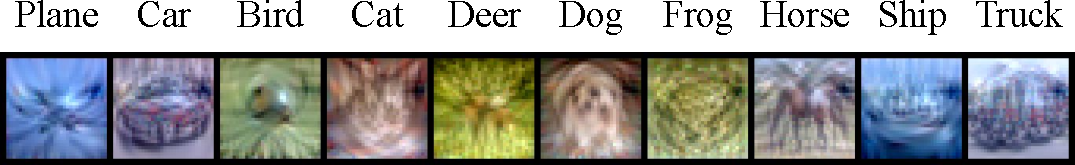
\includegraphics[width=0.88\linewidth]{figures/CIFAR10_1_ipc.pdf}\\[-0.6ex]
    {\smaller 1 image per class} \vspace{0.5cm}\\
        \vspace{-0.34cm}

    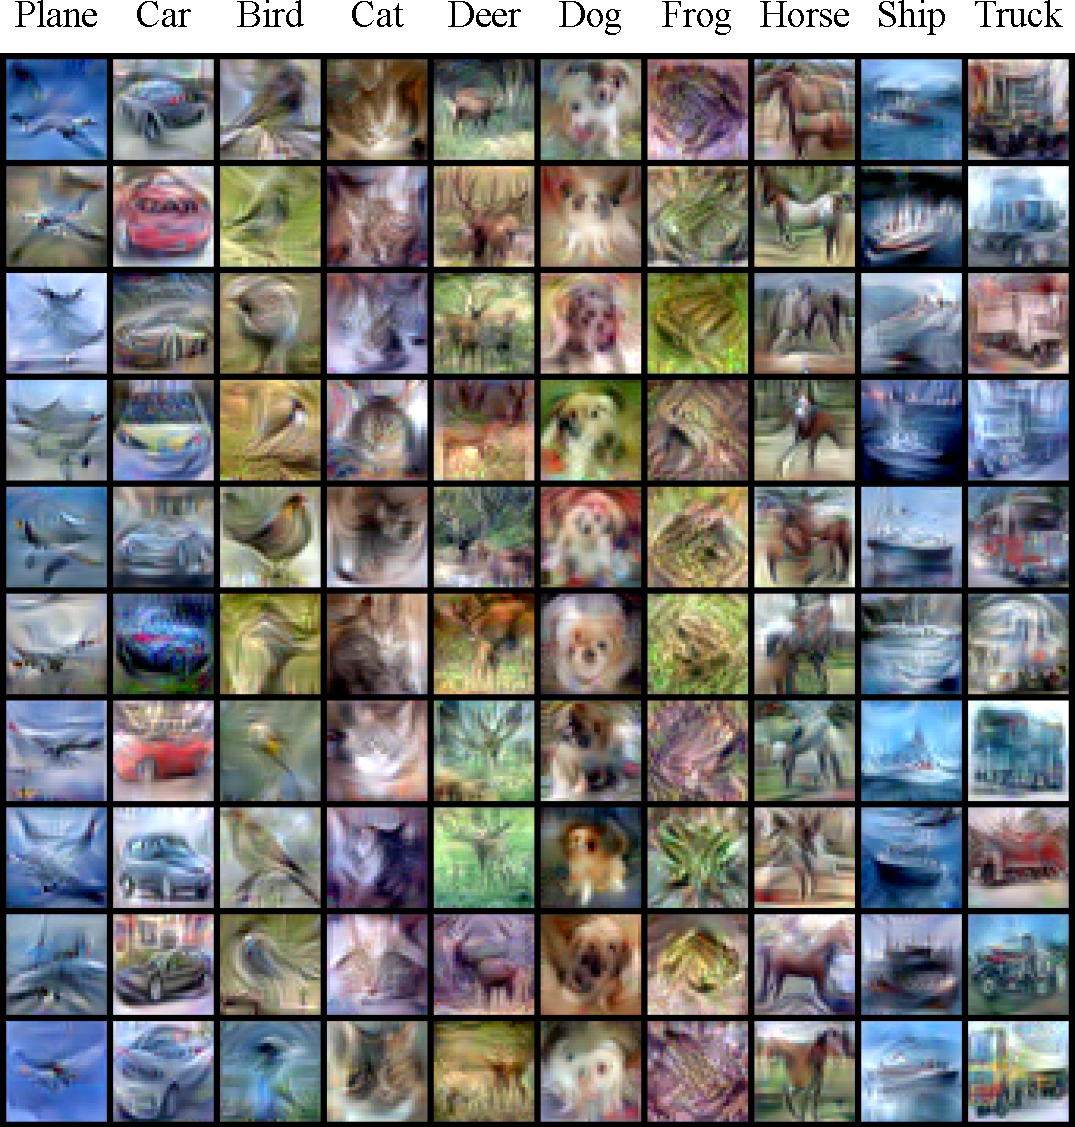
\includegraphics[width=0.88\linewidth, trim=0 0 0 20, clip]{figures/CIFAR10.pdf}\\[-0.6ex]
    {\smaller 10 images per class}
         \vspace{-7pt}
    \caption{CIFAR-10: The 1 image per class images are more abstract but also more information-dense while the 10 images per class images are more expressive and contain more structure.}
    \lblfig{CIFAR-10}
         \vspace{-7pt}
\end{figure}


\subsection{Short-Range vs.~Long-Range Matching}
\lblsec{shortlongrange}

Unlike some prior works (\texttt{DC} and \texttt{DSA}), our method performs long-range parameter matching, where $N$ training steps on distilled data match a much larger $M$ steps on real data. Methods that optimize over entire training processes (\eg \texttt{DD} and \texttt{KIP}) can be viewed as even longer range matching. However, their performances fall short of our method (\eg in \reftbl{sota}), likely due to related instabilities or inexact approximations. Here, we experimentally confirm our hypothesis that long-range matching achieved by larger $M$ and $N$ in our method is superior to the short-range counterparts (such as small $M$ and $N$ and \texttt{DSA}).


In \reffig{mn-alpha} (left), we evaluate our method on different settings of $M$ and $N$. Really short-range matching (with $N=1$ and small $M$) generally exhibits worse performance than long-range matching, with the best performance attained when both $N$ and $M$ are relatively large. Furthermore, as we increase $N$, the power of  $N$ combined steps (on distilled data) becomes stronger and can approximate longer-range behavior, leading to the optimal $M$ values shifting to greater values correspondingly.

\begin{figure}
\vspace{-4pt}
    \begingroup
    \setlength{\tabcolsep}{1pt}
    \centering
    \begin{tabular}{@{\hskip 0pt}cc@{\hskip 0pt}cc@{\hskip 0pt}}
         \rotatebox[origin=c]{90}{\fontsize{6}{5}\selectfont{Validation Acc. \%}} &  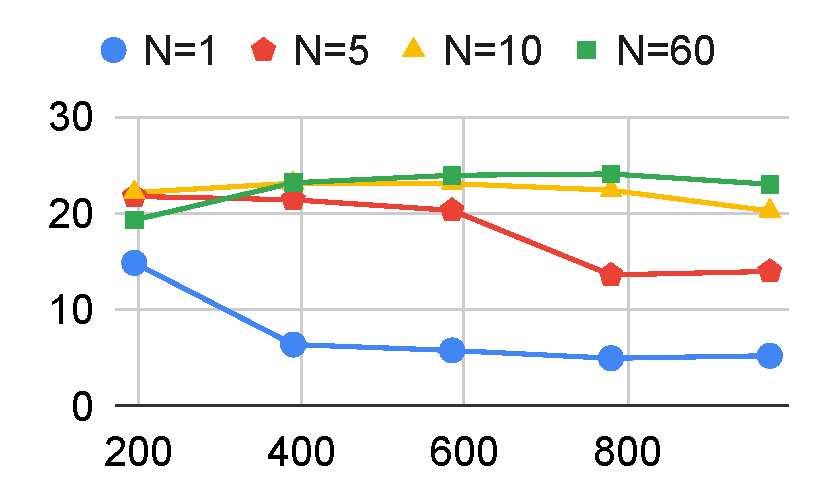
\includegraphics[align=c,width=0.455\linewidth,trim=20 0 0 0,clip]{figures/MandN.pdf}& \hfill\;\;\rotatebox[origin=c]{90}{\fontsize{6}{5}\selectfont{Param. Distance to Target}} &  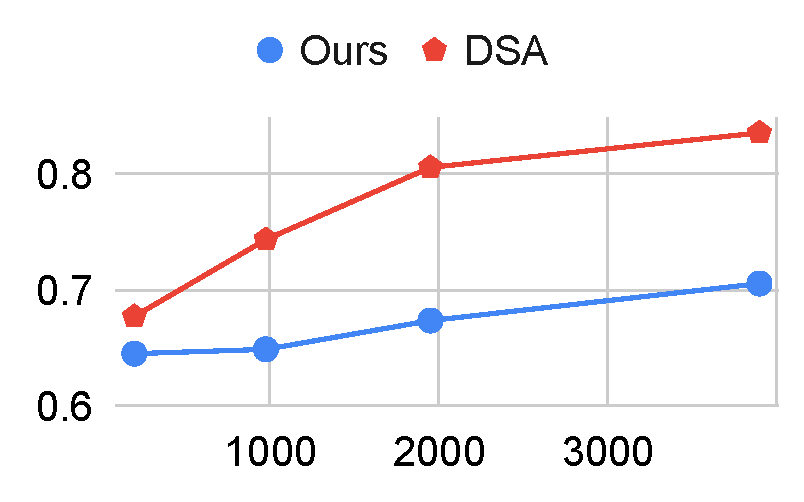
\includegraphics[align=c,width=0.458\linewidth,trim=13 0 9 0,clip]{figures/min_dt.pdf}\\[-1.3ex]
         & \fontsize{6}{5}\selectfont{\;\;\;\;\;$M$: Expert Steps} & & \fontsize{6}{5}\selectfont{\;\;$\Delta t$: Expert Steps between Init.~and Target}
    \end{tabular}
    \endgroup
        \vspace{-9pt}
    \caption{CIFAR-100 (1 image / class). \textbf{Left:} Smaller $M$ and $N$ match shorter-range behavior, which performs worse than longer-range matching. 
    \textbf{Right:} Over $1000$ training steps on distilled data, we track the closest distance in parameter space (normalized MSE in \refeq{weight_matching}) to a target set of parameters, obtained with $\Delta_t$ training steps on real data. Matching long-range behavior, our method better approximate real data training for longer ranges (large $\Delta_t$).
    }
    \lblfig{mn-alpha}
    \vspace{-5pt}
\end{figure}

In  \reffig{mn-alpha} (right), we evaluate our method and a short-range matching work (\texttt{DSA}) on their abilities to approximate real training behavior over short and long ranges. Starting from a set of initial parameters, we set the target parameters to be the result of $\Delta_t$ training steps on real data (\ie the long-range behavior that distilled data should mimic). A small (or large) $\Delta_t$ means evaluating matching over a short (or long) range. For both methods, we test how close they can train the network (using distilled data) from the same initial parameters to the target parameters. \texttt{DSA} is only optimized to match short-range behavior, and thus errors may accumulate during longer training. Indeed, as $\Delta_t$ grows larger, \texttt{DSA} fails to mimic the real data behavior over longer ranges. In comparison, our method is optimized for long-range matching and thus performs much better.







\begin{table}[]
\centering
\resizebox{1\linewidth}{!}{
\begin{tabular}{@{\hskip 2pt}c@{\hskip 4pt}|@{\hskip 5pt}c@{\hskip 5pt}c@{\hskip 5pt}c@{\hskip 5pt}c@{\hskip 5pt}c@{\hskip 5pt}c@{\hskip 0pt}}
\toprule
 & ImageNette & ImageWoof & ImageFruit & ImageMeow & ImageSquawk & ImageYellow \\ \midrule 

1 Img/Cls & 47.7 $\pm$ 0.9 & 28.6 $\pm$ 0.8 & 26.6 $\pm$ 0.8 & 30.7 $\pm $1.6 & 39.4 $\pm$ 1.5 & 45.2 $\pm$ 0.8\\
10  Img/Cls & 63.0 $\pm$ 1.3 & 35.8 $\pm$ 1.8 & 40.3 $\pm$ 1.3 & 40.4 $\pm$ 2.2 & 52.3 $\pm$ 1.0 & 60.0 $\pm$ 1.5\\
                            \midrule
Full Dataset & 87.4 $\pm$ 1.0 & 67.0 $\pm$ 1.3 & 63.9 $\pm$ 2.0 & 66.7 $\pm$ 1.1 & 87.5 $\pm$ 0.3 & 84.4 $\pm$ 0.6\\\bottomrule
\end{tabular}
}
\vspace{-8pt}
\caption{Applying our method to 128$\times$128 resolution ImageNet subsets. On this higher resolution, across various subsets, our method continues to produce high-quality distilled images.}
\lbltbl{imagenet}
     \vspace{-10pt}
\end{table}








\subsection{Tiny ImageNet (64$\times$64)}
\lblsec{tiny}

Introduced to the dataset distillation task by the concurrent work, Distribution Matching (\texttt{DM})~\cite{dm}, we also show the effectiveness of our algorithm on the 200 class, 64$\times$64 Tiny ImageNet~\cite{tiny} dataset (a downscaled subset of ImageNet \cite{deng2009imagenet}). %
To account for the higher image resolution, we move up to a depth-4 ConvNet, similar to \texttt{DM}~\cite{dm}.

Most dataset distillation methods (other than \texttt{DM}) are unable to handle this larger resolution due to extensive memory or time requirement, as the \texttt{DM} authors also observed \citep{dm}. In \reftbl{sota}, our method consistently outperforms the only viable such baseline, \texttt{DM}. Notably, on the 10 images per class task, our method improves the concurrent work \texttt{DM} from  12.9\% and 23.2\%. A subset of our results is shown in \reffig{tinyimagenet}. The supplementary material contains the rest of the images. %


At 200 classes and 64$\times$64 resolution, Tiny ImageNet certainly poses a much harder task than previous datasets. Despite this, many of our distilled images are still recognizable, with a clear color, texture, or shape pattern.
\begin{figure}[t]
    \centering
    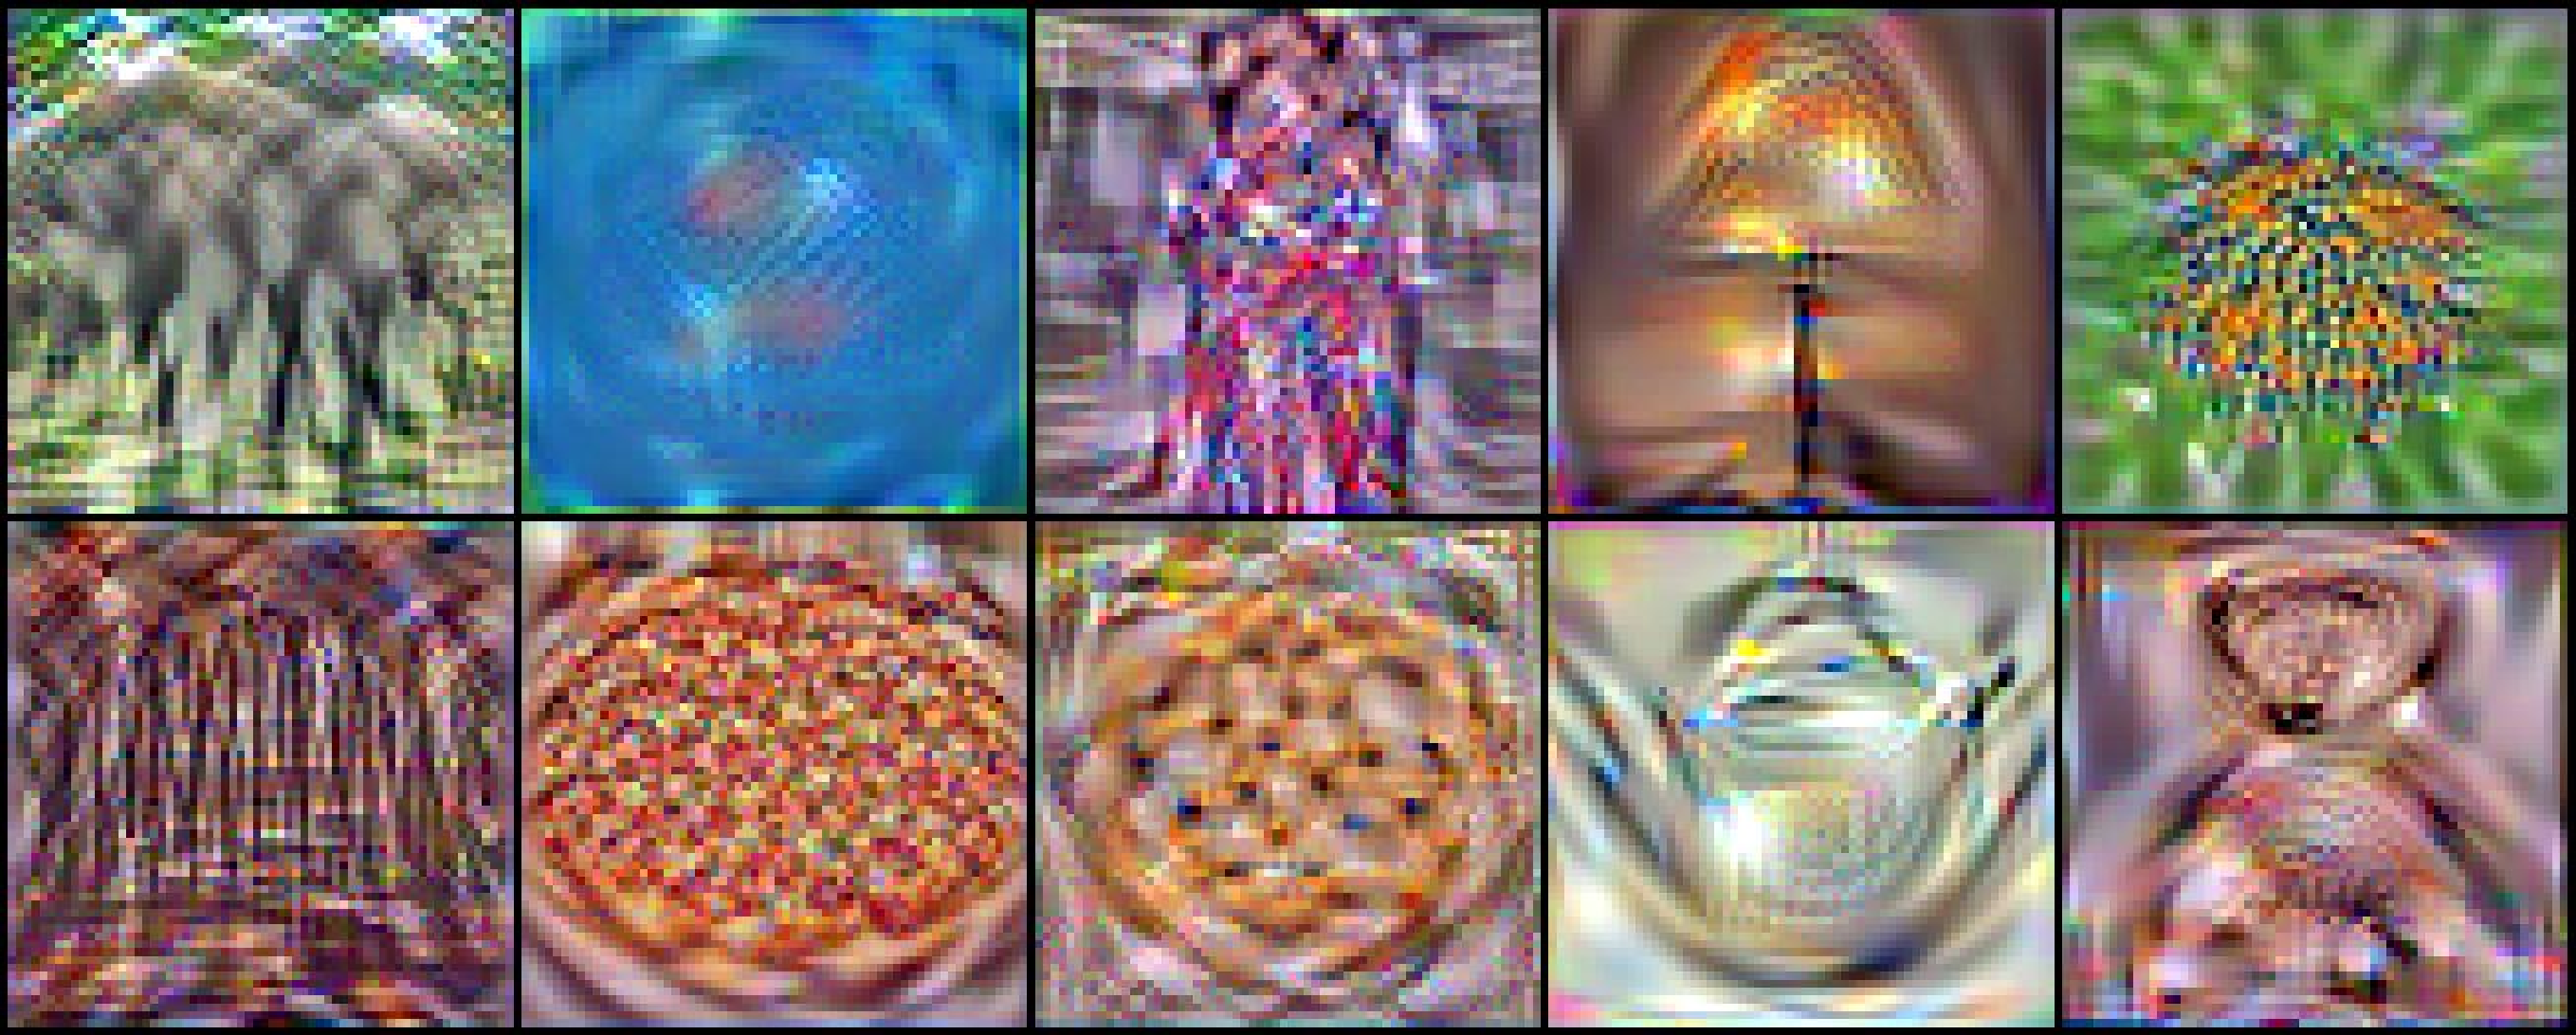
\includegraphics[width=\linewidth]{figures/Tiny.pdf}
         \vspace{-7pt}
    \caption{Selected samples distilled from Tiny ImageNet, one image per class. Despite the higher resolution, our method still produces high-fidelity images. (Can you guess which classes these images represent? Check your answers in the footnote!\protect\footnotemark)}
    \lblfig{tinyimagenet}%
    \vspace{-7pt}
\end{figure}

\footnotetext{\smaller{Answers for \reffig{tinyimagenet}: \textbf{First Row:} African Elephant, Jellyfish, Kimono, Lampshade, Monarch} \textbf{Second Row:} Organ, Pizza, Pretzel, Teapot, Teddy}
\subsection{ImageNet Subsets (128$\times$128)}
\lblsec{imagenet}
\newcommand\imagenetwidth{0.45}
\begin{figure*}[ht]
\vspace{-8pt}
\centering
\begingroup
\setlength{\tabcolsep}{2pt}
\begin{tabular}{cccc}
\rotatebox[origin=c]{90}{\small{ImageNette}}    &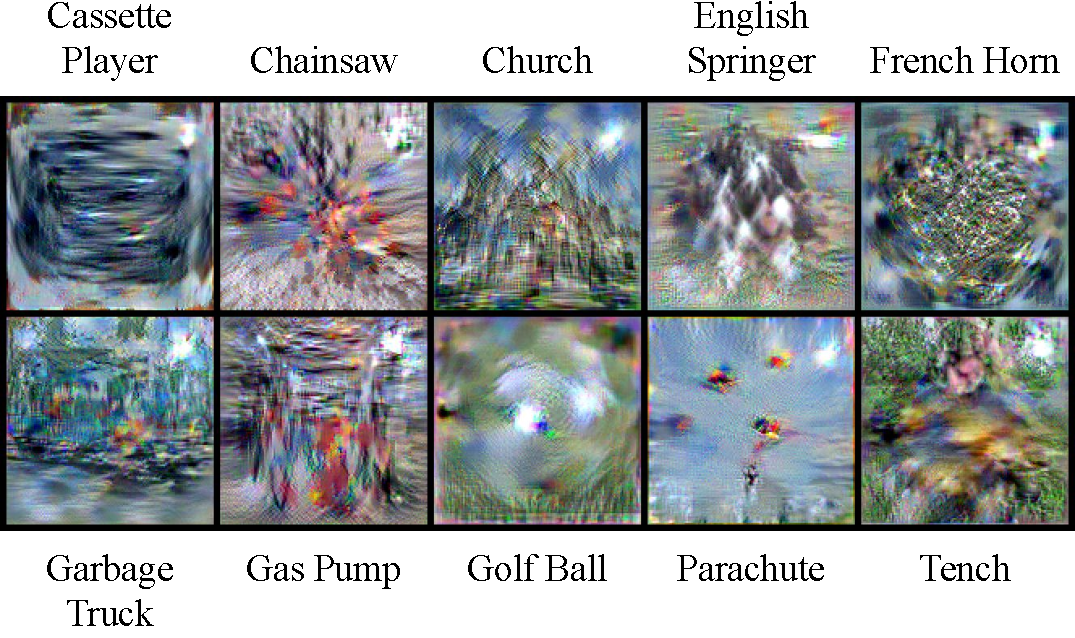
\includegraphics[align=c,width=\imagenetwidth\linewidth]{figures/ImageNette.pdf}
    &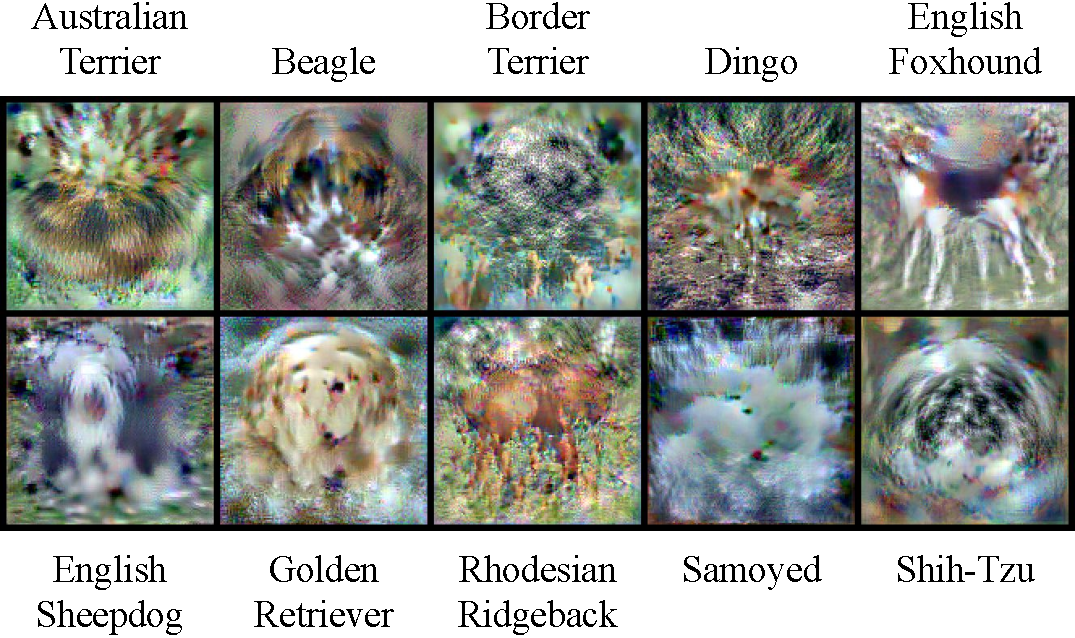
\includegraphics[align=c,width=\imagenetwidth\linewidth]{figures/ImageWoof.pdf} & \rotatebox[origin=c]{270}{\small{ImageWoof}} \\[-0.8ex]
\rotatebox[origin=c]{90}{\small{ImageSquawk}}    &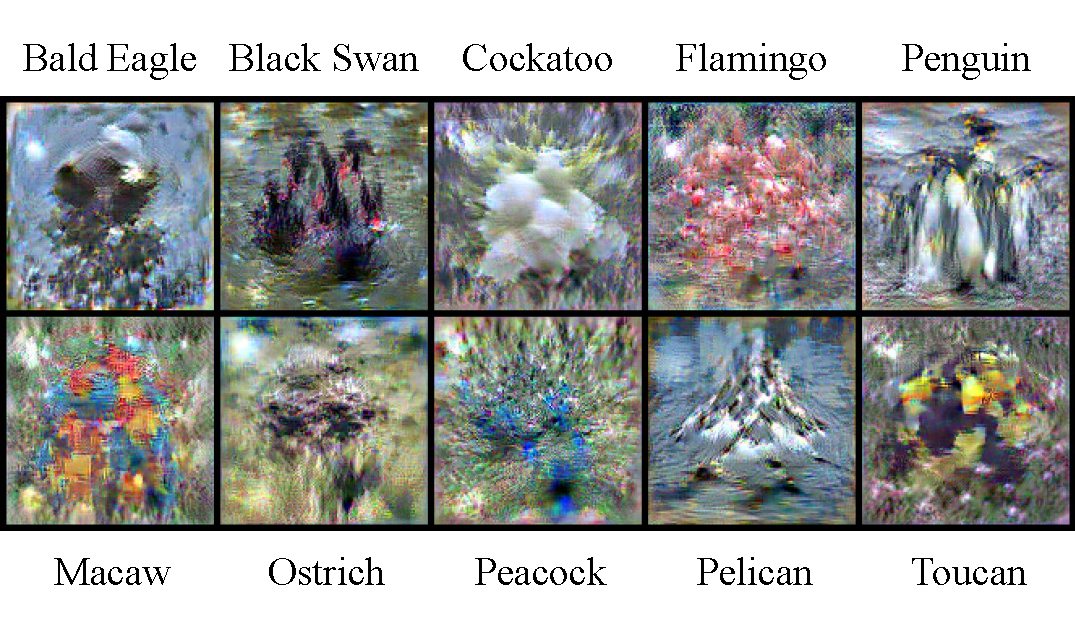
\includegraphics[align=c,width=\imagenetwidth\linewidth]{figures/ImageSquawk.pdf}
    &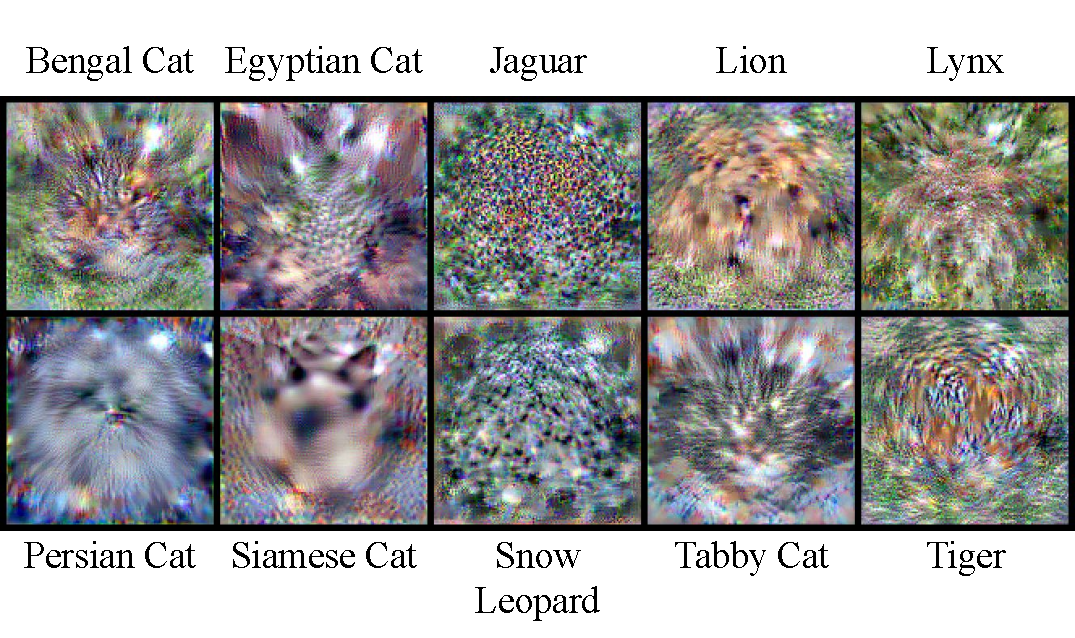
\includegraphics[align=c,width=\imagenetwidth\linewidth]{figures/ImageMeow.pdf} & \rotatebox[origin=c]{270}{\small{ImageMeow}} \\[-0.8ex]
\rotatebox[origin=c]{90}{\small{ImageFruit}}    &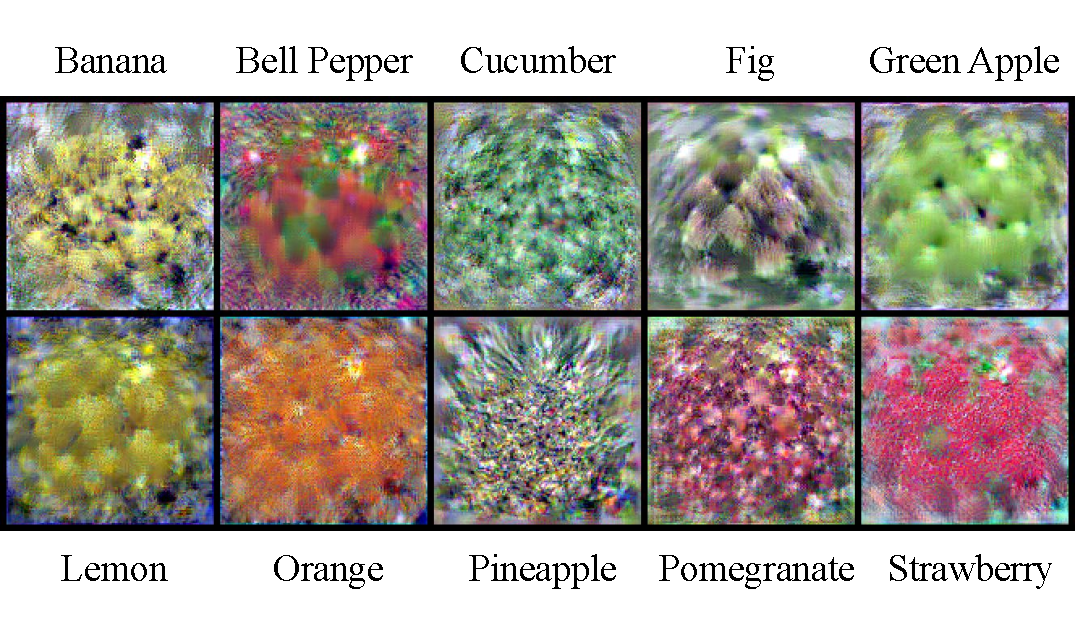
\includegraphics[align=c,width=\imagenetwidth\linewidth]{figures/ImageFruit.pdf}
    &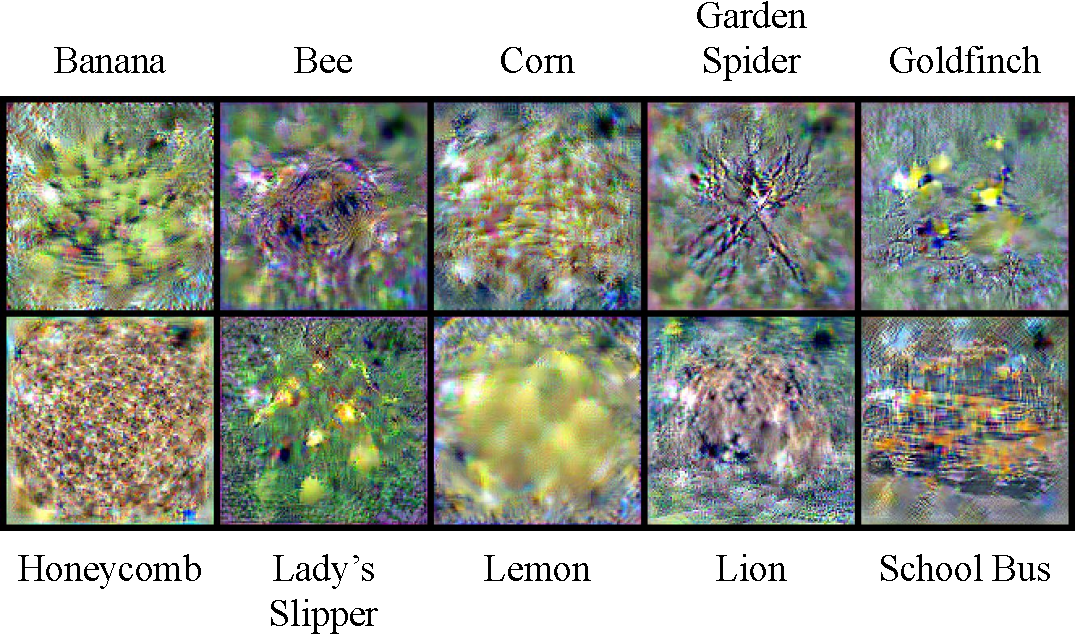
\includegraphics[align=c,width=\imagenetwidth\linewidth]{figures/ImageYellow.pdf} & \rotatebox[origin=c]{270}{\small{ImageYellow}}
\end{tabular}
\endgroup
\vspace{-0.3cm}
    \captionof{figure}{Our method is the first capable of distilling higher-resolution (128$\times$128) images, allowing us to explore the ImageNet \cite{deng2009imagenet} dataset.}
    \lblfig{imagenet}
    \vspace{-6pt}
\end{figure*}


Next, we push the boundaries of dataset distillation even further by running our method on yet higher resolution images in the form of 128$\times$128 subsets of ImageNet~\cite{deng2009imagenet}. Again, due to the higher resolution, we increase the depth of our architecture and use a depth-5 ConvNet for the 128$\times$128 ImageNet subsets.


ImageNette (assorted objects) and ImageWoof (dog breeds) are existing subsets~\cite{imagenette} designed to be easy and hard to learn respectively. We also introduce ImageFruit (fruits), ImageMeow (cats), ImageSquawk (birds), and ImageYellow (yellow-ish things) to further illustrate our algorithm. %

Similar to Tiny ImageNet, most dataset distillation baselines do not scale up to our ImageNet subset settings.
As the code of \texttt{DM}~\cite{dm} is not publicly available now, we choose to only compare to the networks trained on the full dataset. We wish to show that our method transfers well to large images and still produces meaningful results at a higher resolution. Validation set accuracies are presented in \reftbl{imagenet}.

While all of the generated images are devoid of high-frequency noise, the tasks still differ in the type of distilled image they induce. For tasks where all the classes have a similar structure but unique textures like ImageSquawk (\reffig{imagenet}), the distilled images may not have much structure but instead store discriminating information in the textures.

Conversely, for tasks where all classes have similar color or textures like ImageYellow (\reffig{imagenet}), the distilled images seem to diverge from their common trait and accentuate the structure or secondary color that makes them unique. Specifically, note the differences between the distilled ``Banana'' images for the ImageFruit and ImageYellow (bottom row, \reffig{imagenet}). Although the expert trajectory-generating networks saw the same ``Banana'' training images, the distilled images differ between the two tasks. The distilled ``Banana'' for the ImageYellow task is clearly much ``greener'' than the equivalent image for the ImageFruit task. This implies that the expert networks identify different features by which to identify classes based on the other classes in the task.

\end{document}


















